\section {User manual}

\subsection {Introduction}

YaJTris is a clone of the still popular Russian computer game \href{http://en.wikipedia.org/wiki/Tetris}{Tetris} by Alexey Pajitnov in 1985.
YaJTris is written in the Java programming language and is thus portable to a wide range of systems that are supported
by the Java Runtime Environment (JRE).

\subsection {Installation}

YaJTris is distributed in a zip-package. The package contains sources, documentation and a
ready-to-run jar file. YaJTris has been precompiled with Sun Java version 1.5.0 (Java 5 SE) and thus
should run on all runtimes from 1.5 and up. It may work with non-Sun implementations but it has only been tested
with Sun's implementation.

To install YaJTris just extract the package to desired location.

\subsection {Running}

The distribution contains scripts to start YaJTris.

For Windows platforms a script yajtris.bat
is provided and double clicking it on explorer should start the game.

For UNIX platforms there's yajtris.sh. First make sure that the script is executable with command
``chmod +x yajtris''. After that you can start YaJTris with command ``./yajtris.sh''. If this fails
make sure that 'java' program is found in path or that JAVA\_HOME is set to the location of
your Java installation. Refer to Sun's Java installation documentation if in trouble.

You can also try starting YaJTris manually with command: 'java -jar yatris.jar'.

\subsection {Playing}

YaJTris is played on a board of 10x20 squares. The objective is to place tetrominoes
(7 distinct pieces made from 4 squares) one at a time on the board into lines which, when completed, are
cleared from the board. The pieces drop from the upper edge of the board at a steady rate determined by the current level.
These pieces never run out, but the space on board will so make sure you keep the board clean and organized.
The game ends when a piece no longer can drop freely from the upper edge of the board.

As most tetris clones YaJTris makes use of the cursor keys to move the tetromino. Use
the LEFT and RIGHT keys to move the piece left and right respectively. Use the 'UP' key to
rotate the piece and 'DOWN' key to move the piece down faster. To drop the piece press 'SPACE'.

To make things more interesting the player is awarded points for every cleared line. These points
are determined by the current level and the number of lines cleared at a time.

The game partly implements the scoring system used in the Nintendo Tetris as specified at \\
\href{http://www.tetrisconcept.com/wiki/index.php?title=Scoring\#Original_Nintendo_scoring_system}{Original nintendo scoring}.
The scoring scheme is as follows: for one line you score 40*(level+1) points, for two lines 100*(level+1), for three lines 300*(level+1) and
for four lines 1200*(level+1).

When the game ends and you make it to the top ten you'll be prompted for initials (3 characters).

To exit the game press 'ESCAPE' to end the current game. And press 'ESCAPE' again
when the screen says ``Press escape to exit''. You may need to input initials
to be entered into the high scores list before this.

Word of warning: The game is known to be very addictive so make sure you don't have anything urgent to do before
you start playing!

\begin{center}
  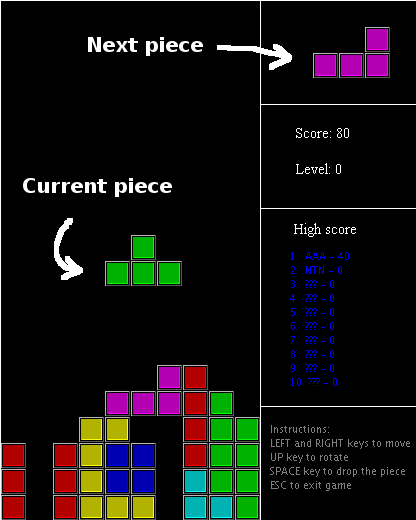
\includegraphics[scale=0.5]{screenshot.png}
\end{center}

\subsection {Compiling}

If you wish to recompile YaJTris there's GNU Makefiles provided to help with the compilation.
On a system with GNU make run 'make' in the root of the YaJTris distribution.

On Windows systems without GNU make you can compile YaJTris manually with 'javac'. Change to the
source directory and run 'javac Game.java'. This should produce the necessary java .class files to
start the game or produce a .jar file. To create a jar-file run the command:
'jar cvfm yajtris.jar manifest *.class'.
